\cleardoublepage \phantomsection
%\addcontentsline{toc}{chapter}{Introduction}
\chapter{The Finite Element Method}
\section{Brief review of the linearized theory of elasticity}
Discuss:
\begin{itemize}
\item Equilibrium equations.
\item Generalized Hooke's law.
\item Strain-displacement rlationships.
\item Equilibrium in terms of displacements (Navier equations) and boundary conditions.
\end{itemize}

\subsection*{Self equilibrated wedge in plane stress}

\section{Formal definition of strong and weak forms}

\subsection{The principle of virtual work}

\section{Discretization of the PVW via the finite element method}
\subsection*{Application to a simple spring-mass system}

\section{Variational formulations}
\subsection{Principle of minimum potential energy}
\subsection{Hu-Washizu Variational Principle}
Consider the followwing functional;

\begin{equation}
{\pi ^*} = \pi  - \int\limits_V {\lambda _{ij}^\varepsilon ({\varepsilon _{ij}} - {L_{ijk}}{u_k})dV}  - \int\limits_{{S_u}} {\lambda _i^u(u_i^{{S_u}} - {{\bar u}_i})dS}
\label{Hu}
\end{equation}

where;

\begin{itemize}
\item $\pi$: is the potential energy functional.
\item $L_{ijk}$ is a differential operator such ${\varepsilon _{ij}} = {L_{ijk}}{u_k}$.
\item $S_u$ surface where esential bundary conditions are prescribed.
\item $\lambda _{ij}^\varepsilon $ and ${\lambda _i^u}$ are Lagrange multipliers.
\end{itemize}

we want to determine the so-called Euler equations resulting from the condition $\delta \pi^* = 0$. Aplying the variational operator we have:

\begin{equation}
\begin{aligned}
\delta \pi *& = \delta \pi  - \int\limits_V {\delta \lambda _{ij}^\varepsilon } ({\varepsilon _{ij}} - {L_{ijk}}{u_k})dV- \int\limits_V {\lambda _{ij}^\varepsilon } (\delta {\varepsilon _{ij}} - {L_{ijk}}\delta {u_k})dV \\
&-\int\limits_V {\delta \lambda _i^u} (u_i^{{S_u}} - {\bar u_i})dS - \int\limits_V {\lambda _i^u} \delta u_i^{{S_u}}dS
\end{aligned}
\end{equation}

\begin{equation}
\begin{aligned}
\delta \pi * &= \int\limits_V {{C_{ijkl}}{\varepsilon _{kl}}\delta {\varepsilon _{ij}}dV - \int\limits_{{S_t}} {{t_i}\delta {u_i}dS}  - \int\limits_V {{f_i}\delta {u_i}dV - } }\int\limits_V {\lambda _{ij}^\varepsilon \delta {\varepsilon _{ij}}dV}  + \int\limits_V {\lambda _{ij}^\varepsilon {L_{ijk}}\delta {u_k}dV}\\
&- \int\limits_V {\delta \lambda _{ij}^\varepsilon ({\varepsilon _{ij}} - {L_{ijk}}{u_k})dV - \int\limits_S {\delta \lambda _i^u(u_i^{{S_u}} - {{\bar u}_i})dS - \int\limits_{{S_u}} {\lambda _i^u\delta {u_i}dS = 0} } }
\end{aligned}
\end{equation}

using

\[\int\limits_V {(\lambda _{ij}^\varepsilon \delta {u_i}){,_j}dV = } \int\limits_V {\lambda _{ij}^\varepsilon \delta {u_{i,j}}dV}  + \int\limits_V {\lambda _{ij,j}^\varepsilon \delta {u_i}dV} \]

in the above we can write

\begin{align*}
\int\limits_V {\lambda _{ij}^\varepsilon {L_{ijk}}\delta {u_k}dV} & = \int\limits_V {{{(\lambda _{ij}^\varepsilon \delta {u_i})}_{,j}}dV}  - \int\limits_V {\lambda _{ij,j}^\varepsilon \delta {u_i}dV}\\
& = \int\limits_{{S_t}} {\lambda _{ij}^\varepsilon \delta {u_i}{{\hat n}_j}dS}  - \int\limits_V {\lambda _{ij,j}^\varepsilon \delta {u_i}dV}
\end{align*}

therefore


\begin{align*}
\delta \pi * &= \int\limits_V {({C_{ijkl}}{\varepsilon _{kl}} - \lambda _{ij}^\varepsilon )\delta {\varepsilon _{ij}}dV - \int\limits_{{S_t}} {{t_i}\delta {u_i}dS}  - \int\limits_V {{f_i}\delta {u_i}dV + } } \int\limits_{{S_t}} {\lambda _{ij}^\varepsilon \delta {u_i}{{\hat n}_j}dS}  - \int\limits_V {\lambda _{ij,j}^\varepsilon \delta {u_i}dV}\\
&- \int\limits_V {\delta \lambda _{ij}^\varepsilon ({\varepsilon _{ij}} - {L_{ijk}}{u_k})dV}  - \int\limits_{{S_u}} {\delta \lambda _i^u(u_i^{{S_u}} - {{\bar u}_i})dS}  - \int\limits_{{S_u}} {\lambda _i^u\delta {u_i}dS}  = 0
\end{align*}


\begin{align*}
&\int\limits_V {({C_{ijkl}}{\varepsilon _{kl}} - \lambda _{ij}^\varepsilon )\delta {\varepsilon _{ij}}dV
+ \int\limits_{{S_t}} {(\lambda _{ij}^\varepsilon {{\hat n}_j} - {t_i})\delta {u_i}dS}  - }\\
&\int\limits_V {(\lambda _{ij,j}^\varepsilon  + {f_i})\delta {u_i}dV}
- \int\limits_V {({\varepsilon _{ij}} - {L_{ijk}}{u_k})\delta \lambda _{ij}^\varepsilon dV}
- \int\limits_{{S_u}} {(u_i^{{S_u}} - {{\bar u}_i})\delta \lambda _i^udS}  - \cancel{\int\limits_{{S_u}} {\lambda _i^u\delta u_i^{{S_u}}dS} = } 0
\end{align*}


Now imposing the conditions $\delta {\varepsilon _{ij}} \neq 0$, $\delta \lambda _{ij}^\varepsilon  \neq 0$, $\delta {u_i} \neq 0$ in $S_t$, $\delta {u_i} \neq 0$ in $V$ and $\delta \lambda _i^u \neq 0$ in $S_u$ we have;

we have

\begin{equation}
\lambda _{ij}^\varepsilon  = {C_{ijkl}}{\varepsilon _{kl}}
\end{equation}



\begin{equation}
{\varepsilon _{ij}} = {L_{ijk}}{u_k}
\end{equation}



\begin{equation}
{t_i} = \lambda _{ij}^\varepsilon {{\hat n}_j}
\end{equation}



\begin{equation}
\lambda _{ij,j}^\varepsilon  + {f_i} = 0
\end{equation}



\begin{equation}
u_i^{{S_u}} = {{\bar u}_i}
\end{equation}

\section{Weighted residual methods}
\subsection{Application to the Navier equtions}
\subsection{Application to the acoustic wave equation}

\section{Basic elements of interpolation theory}
\subsection{Formulation in the physical space}
\subsection{Formulation in the natural space-The continnum mechanics analogy}
In typical finite element equilibrium equations we need to perform integration over the reference element domain $V_0(\vec{x})$ corresponding to originally arbitrarily shaped sub-domains as created during the meshing process.  In order to proceed with this integration it is useful to consider the following continuum mechanics analogy.

First assume that the actual physical domain $V_0(\vec{x})$ is the result of a deformation process imparted upon the natural domain as shown in \cref{fig:natural domain}. In this analogy, the physical domain $V_0(\vec{x})$ is regarded like a "deformed" configuration at an imaginary time $t=t$, while the natural "un-deformed" domain $V(\vec{r})$   is treated like a reference un-deformed configurations at time $t=0$. Both configurations are assumed to be connected through a deformation process;


\begin{equation}
\begin{aligned}
\vec{X}&=\vec{X}(\vec{r})\\
\vec{r}&=\vec{r}(\vec{X})
\end{aligned}
\label{motion}
\end{equation}

\begin{figure}[h]
\centering
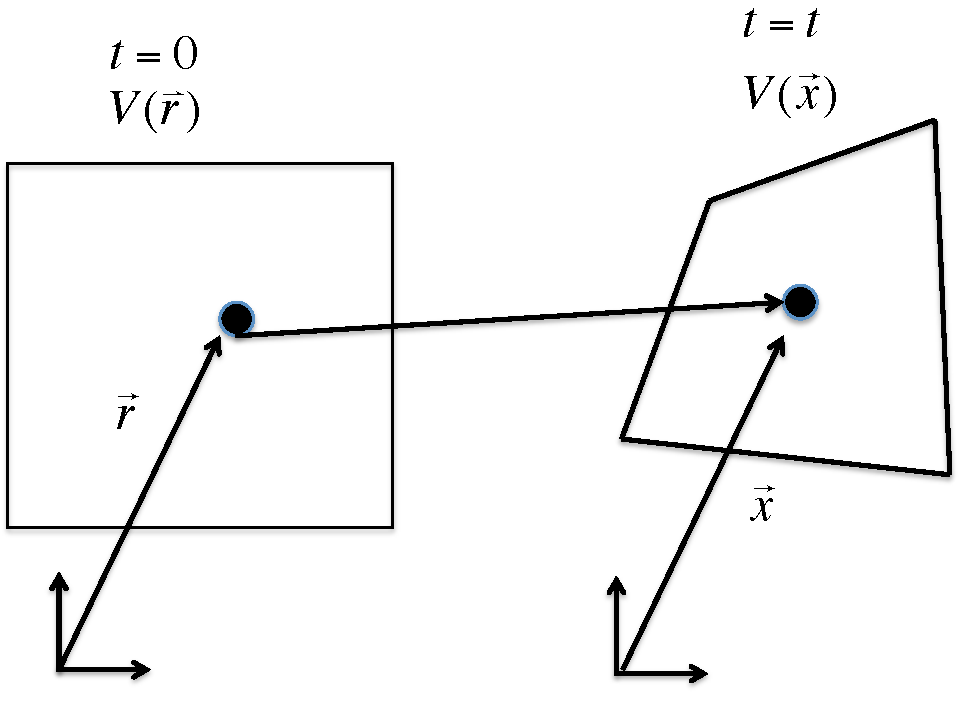
\includegraphics[width=8cm]{img/figure1.pdf}
\caption{Definition of the natural domain}
\label{fig:natural domain}
\end{figure}

 

In \cref{motion} we can understand $\vec{r}$ like a material (Lagrangian) variable and $\vec{X}$ like a spatial (or Eulerian) variable. Using the continuum mechanics analogy it is clear that the "deformation" process at the continuum level is fully characterized by the "deformation" gradient or Jacobian of the transformation \cref{motion} and defined according to;

\begin{equation}
dX_i=\dfrac{\partial X_i}{\partial r_J}dr_J\equiv J_{iJ}dr_{J}
\label{gradient}
\end{equation}

where $dr_{J}$ and $dX_i$ represent material vectors in the original and deformed configuration. From \cref{gradient} it is evident that the Jacobian contains all the information describing the change of the physical sub-domain with respect to the natural element. For the element integration process we will assume that every element $V(\vec{r})$ in the natural domain deforms into the physical element $V_0(\vec{X})$, thus allowing us to write typical terms like the ones in the material stiffness matrix;

\begin{equation}
\int\limits_{V(\vec{X})} \hat{B}_{ij}^K(\vec{X}) C_{ijkl} \hat{B}_{kl}^P(\vec{X}) dV(\vec{X})\equiv \int\limits_{V_0(\vec{r})} \hat{B}_{ij}^K(\vec{r}) C_{ijkl} \hat{B}_{kl}^P(\vec{r})J dV_0(\vec{r})
\label{matmatrix}
\end{equation}


where we have used $dV(\vec{X})=JdV(\vec{r})$, with $J$ being the determinant of the deformation gradient and in general we transform functions between the natural and physical space making use of \cref{motion} according to;

\begin{equation}
f(\vec{r})=F[\vec{X}(\vec{r})]
\label{funtrans}
\end{equation}

	 								
\section*{Interpolation scheme}
Having identified the fact that the integration process will take place in the natural domain, we will approach the interpolation process directly in this natural space. In the case of the displacement based finite element method all the involved variables will then be obtained via interpolation of nodal displacements. For instance, assume that a given problem variable is defined in the physical space by the tensor $\Phi_{ik...p}(\vec{X})$. The interpolated variable is then written like;

\begin{equation}
\Phi_{ij...p}(\vec{X})=H_{ij...p}^K(\vec{r})\hat{u}^K
\label{interpol}
\end{equation}	 						

where $\hat{u}^K$ represents a vector of nodal points displacements, see \cref{fig:interpol nat dom}, and $H_{ij...p}^K(\vec{r})$ is an interpolator which keeps the tensorial character of the original physical variable $\Phi_{ik...p}(\vec{X})$ and where the super-index makes reference to a nodal identifier (with the summation convention in place).


\begin{figure}[h]
\centering
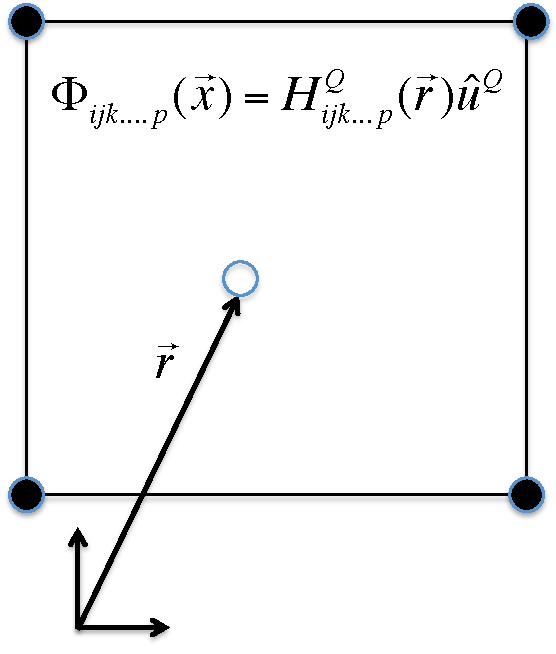
\includegraphics[width=4cm]{img/figure2.pdf}
\caption{General interpolation strategy in the natural domain}
\label{fig:interpol nat dom}
\end{figure}
 


Since the primary variable corresponds to displacements it must be kept in mind that $H_{ij...p}^K(\vec{r})$ corresponds to combinations of derivatives (or other arbitrary combinations) of the basic element shape functions defined in;


\begin{equation}
u_i(\vec{X})=N_i^K(\vec{r})\hat{u}^K
\label{el interpol}
\end{equation}



For the general interpolation process we need two kinds of transformations.  First we need to transform integrals over the physical space into integrals into the natural space which corresponds to;


\begin{equation}
\int\limits_{V(\vec{X})} F(\vec{X})dV(\vec{X})\equiv \int\limits_{V_0(\vec{r})} f(\vec{r})J dV_0(\vec{r})
\label{gen trans}
\end{equation}



Second we need to relate spatial differentiation in both, the physical and spatial domains.  Let us define these operators like $\bigtriangledown_i^X$ and $\bigtriangledown_I^r$ respectively. It then follows from \cref{funtrans} that;

\begin{equation}
\dfrac{\partial F}{\partial X_i}=\dfrac{\partial f}{\partial r_J}\dfrac{\partial r_J}{\partial X_i}
\label{chain}
\end{equation}

from where we can establish the connection between the two operators like


\begin{equation}
\bigtriangledown_i^X=J_{iJ}^{-1}\bigtriangledown_J^r
\label{fundamental}
\end{equation}


\section*{The fundamental interpolator}
We further define the fundamental interpolator giving rise to gradients of the primary displacement variable in the physical space according to;


\begin{equation}
u_{i,j}(\vec{X})=L_{ij}^K(\vec{r})\hat{u}^K
\label{fund operator}
\end{equation}


This fundamental interpolator  $L_{ik}^K(\vec{r})$ is derived after using \cref{el interpol} and \cref{fundamental} in the physical displacement gradient definition as shown next;


\[
\begin{aligned}
u_{i,j}(\vec{X})&=\bigtriangledown_j^X u_i(\vec{X})\\
u_{i,j}(\vec{X})&=\bigtriangledown_j^X N_i^K(\vec{r})\hat{u}^K\\
u_{i,j}(\vec{X})&=J_{jQ}^{-1}\bigtriangledown_Q^r N_i^K(\vec{r})\hat{u}^K\\
u_{i,j}(\vec{X})&=J_{jQ}^{-1}N_{i,Q}^K(\vec{r})\hat{u}^K
\end{aligned}
\]

then

\begin{equation}
L_{ij}^K(\vec{r})=J_{jQ}^{-1}N_{i,Q}^K(\vec{r})
\label{fundamental interpolator}
\end{equation}

\section*{Elemental stiffness matrix}
The elemental material stiffness matrix computed in the natural domain of \cref{fig:Nat domain} reads;

\begin{equation}
K^{KP}=\int\limits_{V_0(\vec{r})} \hat{B}_{ij}^K(\vec{r}) C_{ijkl} \hat{B}_{kl}^P(\vec{r})J dV_0(\vec{r})\equiv \int\limits_{r=-1}^{r=+1}\int\limits_{s=-1}^{s=+1} \hat{B}_{ij}^K(r,s) C_{ijkl} \hat{B}_{kl}^P(r,s)J(r,s) \mathrm{d}r\mathrm{d}s
\label{elematrix}
\end{equation}



\begin{figure}[h]
\centering
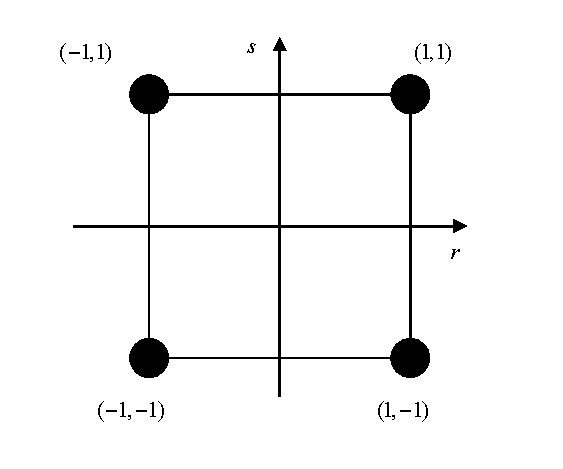
\includegraphics[width=6cm]{img/figure3.pdf}
\caption{Natural domain of integration}
\label{fig:Nat domain}
\end{figure}	 		
 

Once the interpolator $\hat{B}_{ij}^K(\vec{r})$ has been identified the elemental stiffness matrix is obtained via numerical integration (quadrature) as described in \eqref{eleinetgration};

\begin{equation}
\int\limits_{r=-1}^{r=+1}\int\limits_{s=-1}^{s=+1} \hat{B}_{ij}^K(r,s) C_{ijkl} \hat{B}_{kl}^P(r,s)J(r,s) \mathrm{d}r\mathrm{d}s\approx \sum_{i,j=1}^{NGPTS} \alpha_i \alpha_j \hat{B}_{kl}^K(r_i,s_j)C_{ijkl} \hat{B}_{kl}^P(r_i,s_j) J(r_i,s_j)
\label{eleinetgration}
\end{equation}

	 											
and where NGPTS corresponds to the number of integration points, $\alpha_j$ is a weighting factor and $r_i,s_j$   are the coordinates of a typical point $\vec{r}$ in the natural space of \cref{fig:Nat domain}.

 
\begin{figure}[h]
\centering
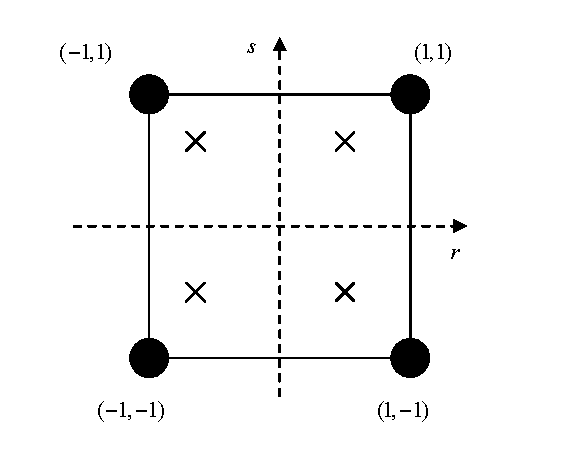
\includegraphics[width=6cm]{img/figure4.pdf}
\caption{Natural integration domain showing quadrature evaluation nodes}
\label{fig:integration domain}
\end{figure}	 


One important aspect of the numerical integration that has to be kept in mind is accuracy.  Depending on the particularly selected integration scheme, the number of introduced integration points fixes the maximum polynomial order of the considered functions that can be integrated accurately.  In the case of the integrand in \cref{eleinetgration}, it is clear that this order increases as the distortion of the physical element  with respect to the natural element increases.  One way of dealing with this dependency of accuracy with element distortion is to make use of adaptative integration techniques which are numerically expensive.  What is actually done in standard FEM analysis is to choose the number of quadrature points beforehand and introduce distortion related error criteria inside the code in such a way that some sort of validation is performed before the numerical integration process is started.

\section*{Strain displacement interpolator for the infinitesimal strain tensor}
The $Q$-th nodal contribution to the infinitesimal strain-displacement interpolator can be obtained in explicit form as follows. Let $L_x^Q$ and $L_y^Q$ be the spatial differential operators in $x$ and $y$ respectively. We have after expanding \cref{fundamental interpolator}  that

\begin{align*}
L_x^Q & = J_{xP}^{ - 1}\frac{{\partial {N^Q}}}{{\partial {r_P}}} \equiv J_{xr}^{ - 1}\frac{{\partial {N^Q}}}{{\partial r}} + J_{xs}^{ - 1}\frac{{\partial {N^Q}}}{{\partial s}}\\
L_y^Q & = J_{yP}^{ - 1}\frac{{\partial {N^Q}}}{{\partial {r_P}}} \equiv J_{yr}^{ - 1}\frac{{\partial {N^Q}}}{{\partial r}} + J_{ys}^{ - 1}\frac{{\partial {N^Q}}}{{\partial s}}
\end{align*}

or in matrix form;

\begin{equation}
\left\{ {\begin{array}{*{20}{c}}
{L_x^Q}\\
{L_y^Q}
\end{array}} \right\} = \left[ {\begin{array}{*{20}{c}}
{J_{xP}^{ - 1}}&{J_{xs}^{ - 1}}\\
{J_{yr}^{ - 1}}&{J_{ys}^{ - 1}}
\end{array}} \right]\left\{ {\begin{array}{*{20}{c}}
{\frac{{\partial {N^Q}}}{{\partial r}}}\\
{\frac{{\partial {N^Q}}}{{\partial s}}}
\end{array}} \right\}
\end{equation}

The $Q$-th nodal contribution is then assembled as follows;


\begin{equation}
\left\{ {\begin{array}{*{20}{c}}
{\frac{{\partial u}}{{\partial x}}}\\
{\frac{{\partial v}}{{\partial y}}}\\
{\frac{{\partial u}}{{\partial y}} + \frac{{\partial v}}{{\partial x}}}
\end{array}} \right\} = \left[ {\begin{array}{*{20}{c}}
.&.&.&{\begin{array}{*{20}{c}}
{L_x^Q}&0\\
0&{L_y^Q}\\
{L_y^Q}&{L_{xy}^Q}
\end{array}}.&.&.&
\end{array}}\right]
\left\{ {\begin{array}{*{20}{c}}
.\\
.\\
.\\
{{u^Q}}\\
{{v^Q}}\\
.\\
.\\
.
\end{array}} \right\}
\label{strain inter}
\end{equation}

\begin{algorithm}[H]
\SetAlgoLined
\KwData{Nodal coordinates $x^Q$}
\KwResult{Strain-displacement interpolator $B_{ij}^Q$ }
Compute Jacobian ${J_{iJ}} = \frac{{\partial N_i^Q}}{{\partial {r_J}}}{{\hat x}^Q}$\\
Invert Jacobian  ${J_{iJ}} \to J_{iJ}^{ - 1}$\\
Compute fundamental interpolator $L_{ij}^Q = J_{jP}^{ - 1}\frac{{\partial N_i^Q}}{{\partial {r_P}}}$\\
Assemble $B_{ij}^Q = \frac{1}{2}\left( {L_{ij}^Q + L_{ji}^Q} \right)$ 
\caption{Strain-displacement interpolator}
\end{algorithm}


